\documentclass[tikz,margin=2mm]{standalone}
\pagestyle{empty}

\usepackage{amsmath}
\usepackage{bm}
\usetikzlibrary{positioning,calc,arrows,arrows.meta}
\tikzset{font=\small}

\begin{document}

	% Example a True DAG
	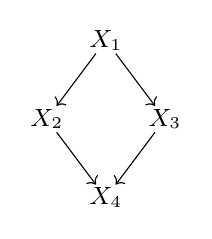
\begin{tikzpicture}
	\begin{scope}
		\tikzstyle{every node}=[align=center, inner sep=1pt]
		\node (x1) at (0, 0) {$X_1$};
		\node (x2) at (-0.75, -1) {$X_2$};
		\node (x3) at (0.75, -1) {$X_3$};
		\node (x4) at (0, -2) {$X_4$};

		\draw[->] (x1) -- (x2);
		\draw[->] (x1) -- (x3);
		\draw[->] (x2) -- (x4);
		\draw[->] (x3) -- (x4);
	\end{scope}
	\end{tikzpicture}

	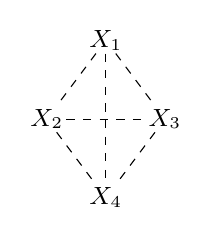
\begin{tikzpicture}
	\begin{scope}
		\tikzstyle{every node}=[align=center, inner sep=1pt]
		\node (x1) at (0, 0) {$X_1$};
		\node (x2) at (-0.75, -1) {$X_2$};
		\node (x3) at (0.75, -1) {$X_3$};
		\node (x4) at (0, -2) {$X_4$};

		\draw[dashed] (x1) -- (x2);
		\draw[dashed] (x1) -- (x3);
		\draw[dashed] (x2) -- (x4);
		\draw[dashed] (x3) -- (x4);
		\draw[dashed] (x1) -- (x4);
		\draw[dashed] (x2) -- (x3);
	\end{scope}
	\end{tikzpicture}

	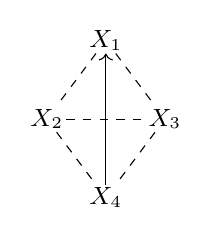
\begin{tikzpicture}
	\begin{scope}
		\tikzstyle{every node}=[align=center, inner sep=1pt]
		\node (x1) at (0, 0) {$X_1$};
		\node (x2) at (-0.75, -1) {$X_2$};
		\node (x3) at (0.75, -1) {$X_3$};
		\node (x4) at (0, -2) {$X_4$};

		\draw[dashed] (x1) -- (x2);
		\draw[dashed] (x1) -- (x3);
		\draw[dashed] (x2) -- (x4);
		\draw[dashed] (x3) -- (x4);
		\draw[->] (x4) -- (x1);
		\draw[dashed] (x2) -- (x3);
	\end{scope}
	\end{tikzpicture}

	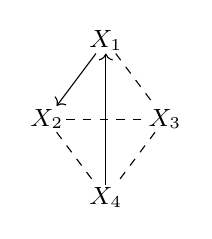
\begin{tikzpicture}
	\begin{scope}
		\tikzstyle{every node}=[align=center, inner sep=1pt]
		\node (x1) at (0, 0) {$X_1$};
		\node (x2) at (-0.75, -1) {$X_2$};
		\node (x3) at (0.75, -1) {$X_3$};
		\node (x4) at (0, -2) {$X_4$};

		\draw[->] (x1) -- (x2);
		\draw[dashed] (x1) -- (x3);
		\draw[dashed] (x2) -- (x4);
		\draw[dashed] (x3) -- (x4);
		\draw[->] (x4) -- (x1);
		\draw[dashed] (x2) -- (x3);

	\end{scope}
	\end{tikzpicture}

	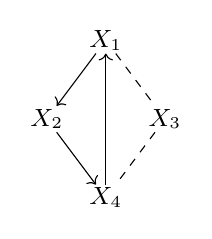
\begin{tikzpicture}
	\begin{scope}
		\tikzstyle{every node}=[align=center, inner sep=1pt]
		\node (x1) at (0, 0) {$X_1$};
		\node (x2) at (-0.75, -1) {$X_2$};
		\node (x3) at (0.75, -1) {$X_3$};
		\node (x4) at (0, -2) {$X_4$};

		\draw[->]     (x1) -- (x2);
		\draw[dashed] (x1) -- (x3);
		\draw[->]     (x2) -- (x4);
		\draw[dashed] (x3) -- (x4);
		\draw[->]     (x4) -- (x1);
	\end{scope}
	\end{tikzpicture}

	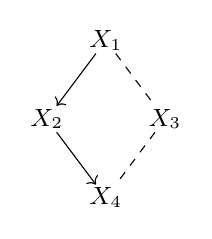
\begin{tikzpicture}
	\begin{scope}
		\tikzstyle{every node}=[align=center, inner sep=1pt]
		\node (x1) at (0, 0) {$X_1$};
		\node (x2) at (-0.75, -1) {$X_2$};
		\node (x3) at (0.75, -1) {$X_3$};
		\node (x4) at (0, -2) {$X_4$};
		
		\draw[->]     (x1) -- (x2);
		\draw[dashed] (x1) -- (x3);
		\draw[->]     (x2) -- (x4);
		\draw[dashed] (x3) -- (x4);
	\end{scope}
	\end{tikzpicture}

	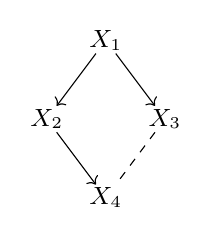
\begin{tikzpicture}
	\begin{scope}
		\tikzstyle{every node}=[align=center, inner sep=1pt]
		\node (x1) at (0, 0) {$X_1$};
		\node (x2) at (-0.75, -1) {$X_2$};
		\node (x3) at (0.75, -1) {$X_3$};
		\node (x4) at (0, -2) {$X_4$};

		\draw[->]     (x1) -- (x2);
		\draw[->]     (x1) -- (x3);
		\draw[->]     (x2) -- (x4);
		\draw[dashed] (x3) -- (x4);
	\end{scope}
	\end{tikzpicture}


	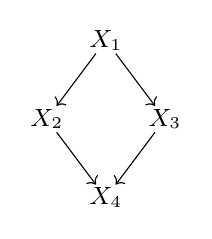
\begin{tikzpicture}
	\begin{scope}
		\tikzstyle{every node}=[align=center, inner sep=1pt]
		\node (x1) at (0, 0) {$X_1$};
		\node (x2) at (-0.75, -1) {$X_2$};
		\node (x3) at (0.75, -1) {$X_3$};
		\node (x4) at (0, -2) {$X_4$};

		\draw[->] (x1) -- (x2);
		\draw[->] (x1) -- (x3);
		\draw[->] (x2) -- (x4);
		\draw[->] (x3) -- (x4);
	\end{scope}
	\end{tikzpicture}

\end{document}
